\documentclass{standalone}
\usepackage{tikz}
\usetikzlibrary{patterns, positioning}


\begin{document}
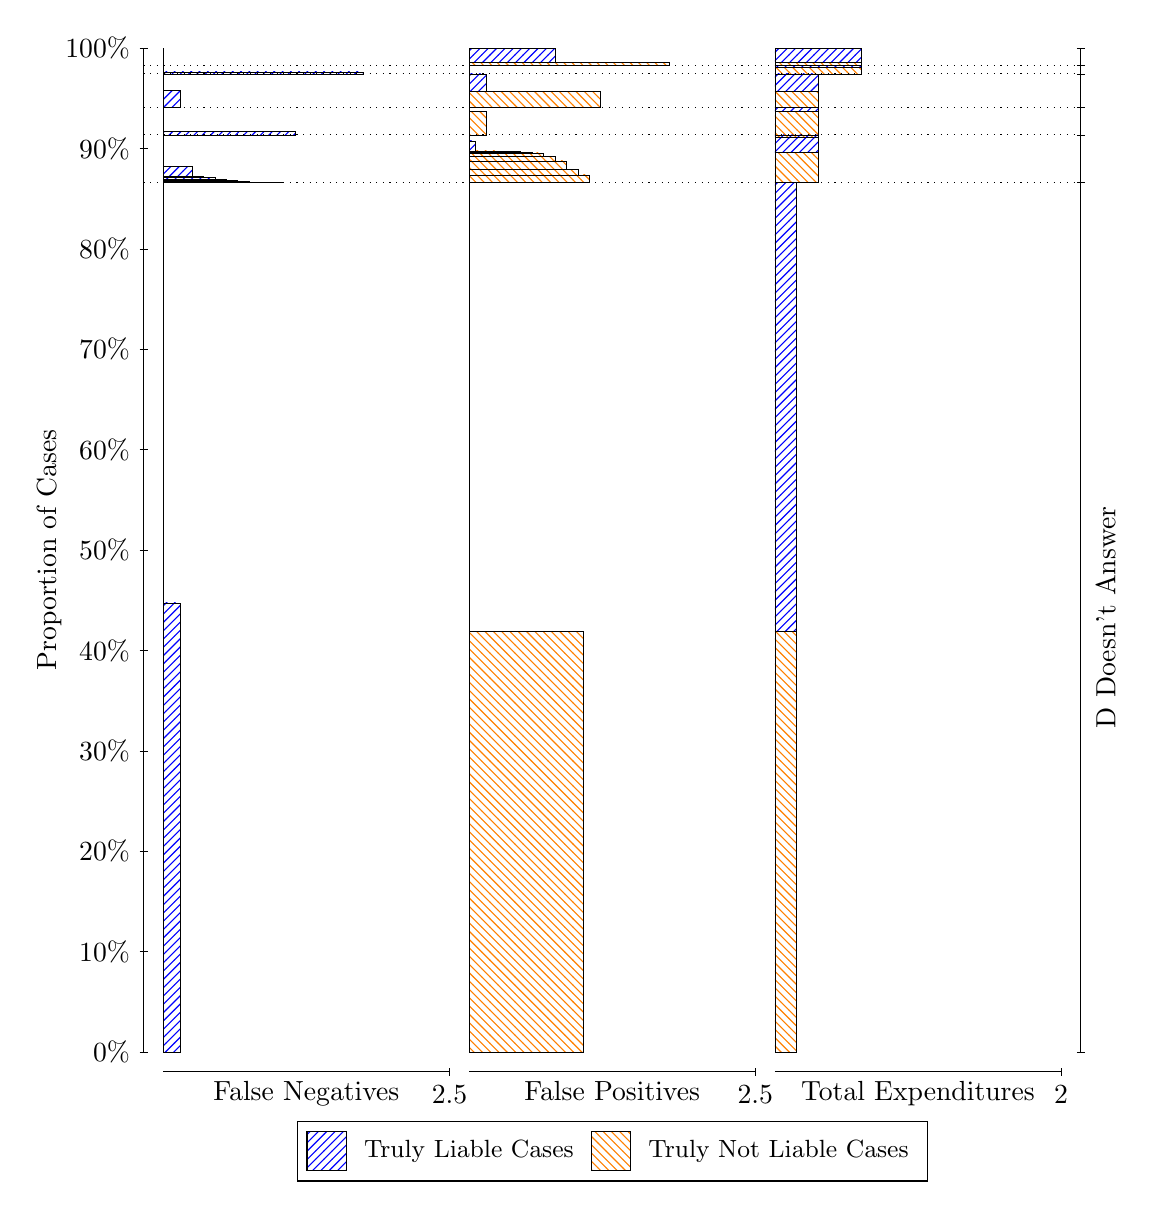
\begin{tikzpicture}
\draw[black, very thin] (1.5,1.75) -- (1.5,14.5);
\node[rotate=90, text=black, anchor=center] at (0.3, 8.125) {Proportion of Cases};
\draw[black, very thin] (1.45,1.75) -- (1.55,1.75);
\node[text=black, anchor=east] at (1.45, 1.75) {0\%};
\draw[black, very thin] (1.45,3.025) -- (1.55,3.025);
\node[text=black, anchor=east] at (1.45, 3.025) {10\%};
\draw[black, very thin] (1.45,4.3) -- (1.55,4.3);
\node[text=black, anchor=east] at (1.45, 4.3) {20\%};
\draw[black, very thin] (1.45,5.575) -- (1.55,5.575);
\node[text=black, anchor=east] at (1.45, 5.575) {30\%};
\draw[black, very thin] (1.45,6.85) -- (1.55,6.85);
\node[text=black, anchor=east] at (1.45, 6.85) {40\%};
\draw[black, very thin] (1.45,8.125) -- (1.55,8.125);
\node[text=black, anchor=east] at (1.45, 8.125) {50\%};
\draw[black, very thin] (1.45,9.4) -- (1.55,9.4);
\node[text=black, anchor=east] at (1.45, 9.4) {60\%};
\draw[black, very thin] (1.45,10.675) -- (1.55,10.675);
\node[text=black, anchor=east] at (1.45, 10.675) {70\%};
\draw[black, very thin] (1.45,11.95) -- (1.55,11.95);
\node[text=black, anchor=east] at (1.45, 11.95) {80\%};
\draw[black, very thin] (1.45,13.225) -- (1.55,13.225);
\node[text=black, anchor=east] at (1.45, 13.225) {90\%};
\draw[black, very thin] (1.45,14.5) -- (1.55,14.5);
\node[text=black, anchor=east] at (1.45, 14.5) {100\%};

\draw[black, very thin] (13.4,1.75) -- (13.4,14.5);
\draw[black, very thin] (13.35,1.75) -- (13.45,1.75);
\node[anchor=west] at (13.35, 1.75) {};
\draw[black, very thin] (13.35,12.79) -- (13.45,12.79);
\node[anchor=west] at (13.35, 12.79) {};
\draw[black, very thin] (13.35,13.398) -- (13.45,13.398);
\node[anchor=west] at (13.35, 13.398) {};
\draw[black, very thin] (13.35,13.746) -- (13.45,13.746);
\node[anchor=west] at (13.35, 13.746) {};
\draw[black, very thin] (13.35,14.171) -- (13.45,14.171);
\node[anchor=west] at (13.35, 14.171) {};
\draw[black, very thin] (13.35,14.282) -- (13.45,14.282);
\node[anchor=west] at (13.35, 14.282) {};
\draw[black, very thin] (13.35,14.5) -- (13.45,14.5);
\node[anchor=west] at (13.35, 14.5) {};

\draw[black, very thin, pattern color=blue, pattern=north east lines] (1.75,1.75) rectangle (1.968,7.4523);
\draw[black, very thin, pattern color=orange, pattern=north west lines] (1.75,7.4523) rectangle (1.75,12.79);
\draw[black, very thin, pattern color=blue, pattern=north east lines] (1.75,12.79) rectangle (3.276,12.792);
\draw[black, very thin, pattern color=blue, pattern=north east lines] (1.75,12.792) rectangle (3.1307,12.794);
\draw[black, very thin, pattern color=blue, pattern=north east lines] (1.75,12.794) rectangle (2.9853,12.798);
\draw[black, very thin, pattern color=blue, pattern=north east lines] (1.75,12.798) rectangle (2.84,12.802);
\draw[black, very thin, pattern color=blue, pattern=north east lines] (1.75,12.802) rectangle (2.6947,12.817);
\draw[black, very thin, pattern color=blue, pattern=north east lines] (1.75,12.817) rectangle (2.5493,12.831);
\draw[black, very thin, pattern color=blue, pattern=north east lines] (1.75,12.831) rectangle (2.404,12.855);
\draw[black, very thin, pattern color=blue, pattern=north east lines] (1.75,12.855) rectangle (2.2587,12.867);
\draw[black, very thin, pattern color=blue, pattern=north east lines] (1.75,12.867) rectangle (2.1133,12.994);
\draw[black, very thin, pattern color=orange, pattern=north west lines] (1.75,12.994) rectangle (1.75,13.398);
\draw[black, very thin, pattern color=blue, pattern=north east lines] (1.75,13.398) rectangle (3.4213,13.443);
\draw[black, very thin, pattern color=orange, pattern=north west lines] (1.75,13.443) rectangle (1.75,13.746);
\draw[black, very thin, pattern color=blue, pattern=north east lines] (1.75,13.746) rectangle (1.968,13.963);
\draw[black, very thin, pattern color=orange, pattern=north west lines] (1.75,13.963) rectangle (1.75,14.171);
\draw[black, very thin, pattern color=blue, pattern=north east lines] (1.75,14.171) rectangle (4.2933,14.197);
\draw[black, very thin, pattern color=orange, pattern=north west lines] (1.75,14.197) rectangle (1.75,14.282);
\draw[black, very thin, pattern color=orange, pattern=north west lines] (1.75,14.282) rectangle (1.75,14.32);
\draw[black, very thin, pattern color=blue, pattern=north east lines] (1.75,14.32) rectangle (1.75,14.5);
\draw[black, very thin, pattern color=orange, pattern=north west lines] (5.6333,1.75) rectangle (7.0867,7.0877);
\draw[black, very thin, pattern color=blue, pattern=north east lines] (5.6333,7.0877) rectangle (5.6333,12.79);
\draw[black, very thin, pattern color=orange, pattern=north west lines] (5.6333,12.79) rectangle (7.1593,12.89);
\draw[black, very thin, pattern color=orange, pattern=north west lines] (5.6333,12.89) rectangle (7.014,12.954);
\draw[black, very thin, pattern color=orange, pattern=north west lines] (5.6333,12.954) rectangle (6.8687,13.066);
\draw[black, very thin, pattern color=orange, pattern=north west lines] (5.6333,13.066) rectangle (6.7233,13.119);
\draw[black, very thin, pattern color=orange, pattern=north west lines] (5.6333,13.119) rectangle (6.578,13.168);
\draw[black, very thin, pattern color=orange, pattern=north west lines] (5.6333,13.168) rectangle (6.4327,13.172);
\draw[black, very thin, pattern color=orange, pattern=north west lines] (5.6333,13.172) rectangle (6.4327,13.177);
\draw[black, very thin, pattern color=orange, pattern=north west lines] (5.6333,13.177) rectangle (6.2873,13.185);
\draw[black, very thin, pattern color=orange, pattern=north west lines] (5.6333,13.185) rectangle (6.142,13.189);
\draw[black, very thin, pattern color=orange, pattern=north west lines] (5.6333,13.189) rectangle (5.9967,13.194);
\draw[black, very thin, pattern color=blue, pattern=north east lines] (5.6333,13.194) rectangle (5.706,13.32);
\draw[black, very thin, pattern color=blue, pattern=north east lines] (5.6333,13.32) rectangle (5.6333,13.398);
\draw[black, very thin, pattern color=orange, pattern=north west lines] (5.6333,13.398) rectangle (5.8513,13.7);
\draw[black, very thin, pattern color=blue, pattern=north east lines] (5.6333,13.7) rectangle (5.6333,13.746);
\draw[black, very thin, pattern color=orange, pattern=north west lines] (5.6333,13.746) rectangle (7.3047,13.954);
\draw[black, very thin, pattern color=blue, pattern=north east lines] (5.6333,13.954) rectangle (5.8513,14.171);
\draw[black, very thin, pattern color=orange, pattern=north west lines] (5.6333,14.171) rectangle (5.6333,14.256);
\draw[black, very thin, pattern color=blue, pattern=north east lines] (5.6333,14.256) rectangle (5.6333,14.282);
\draw[black, very thin, pattern color=orange, pattern=north west lines] (5.6333,14.282) rectangle (8.1767,14.32);
\draw[black, very thin, pattern color=blue, pattern=north east lines] (5.6333,14.32) rectangle (6.7233,14.5);
\draw[black, very thin, pattern color=orange, pattern=north west lines] (9.5167,1.75) rectangle (9.7892,7.0877);
\draw[black, very thin, pattern color=blue, pattern=north east lines] (9.5167,7.0877) rectangle (9.7892,12.79);
\draw[black, very thin, pattern color=orange, pattern=north west lines] (9.5167,12.79) rectangle (10.062,13.172);
\draw[black, very thin, pattern color=blue, pattern=north east lines] (9.5167,13.172) rectangle (10.062,13.366);
\draw[black, very thin, pattern color=orange, pattern=north west lines] (9.5167,13.366) rectangle (10.062,13.37);
\draw[black, very thin, pattern color=blue, pattern=north east lines] (9.5167,13.37) rectangle (10.062,13.372);
\draw[black, very thin, pattern color=orange, pattern=north west lines] (9.5167,13.372) rectangle (10.062,13.39);
\draw[black, very thin, pattern color=blue, pattern=north east lines] (9.5167,13.39) rectangle (10.062,13.398);
\draw[black, very thin, pattern color=orange, pattern=north west lines] (9.5167,13.398) rectangle (10.062,13.7);
\draw[black, very thin, pattern color=blue, pattern=north east lines] (9.5167,13.7) rectangle (10.062,13.746);
\draw[black, very thin, pattern color=orange, pattern=north west lines] (9.5167,13.746) rectangle (10.062,13.954);
\draw[black, very thin, pattern color=blue, pattern=north east lines] (9.5167,13.954) rectangle (10.062,14.171);
\draw[black, very thin, pattern color=orange, pattern=north west lines] (9.5167,14.171) rectangle (10.607,14.256);
\draw[black, very thin, pattern color=blue, pattern=north east lines] (9.5167,14.256) rectangle (10.607,14.282);
\draw[black, very thin, pattern color=orange, pattern=north west lines] (9.5167,14.282) rectangle (10.607,14.32);
\draw[black, very thin, pattern color=blue, pattern=north east lines] (9.5167,14.32) rectangle (10.607,14.5);
\draw[black, dotted] (1.5,12.79) -- (13.4,12.79);
\draw[black, dotted] (1.5,13.398) -- (13.4,13.398);
\draw[black, dotted] (1.5,13.746) -- (13.4,13.746);
\draw[black, dotted] (1.5,14.171) -- (13.4,14.171);
\draw[black, dotted] (1.5,14.282) -- (13.4,14.282);
\draw[black, very thin] (1.75,1.5) -- (5.3833,1.5);
\node[text=black, anchor=north] at (3.5667, 1.5) {False Negatives};
\draw[black, very thin] (5.3833,1.45) -- (5.3833,1.55);
\node[text=black, anchor=north] at (5.3833, 1.45) {2.5};

\draw[black, very thin] (5.6333,1.5) -- (9.2667,1.5);
\node[text=black, anchor=north] at (7.45, 1.5) {False Positives};
\draw[black, very thin] (9.2667,1.45) -- (9.2667,1.55);
\node[text=black, anchor=north] at (9.2667, 1.45) {2.5};

\draw[black, very thin] (9.5167,1.5) -- (13.15,1.5);
\node[text=black, anchor=north] at (11.333, 1.5) {Total Expenditures};
\draw[black, very thin] (13.15,1.45) -- (13.15,1.55);
\node[text=black, anchor=north] at (13.15, 1.45) {2};

\node[text=black, centered, rotate=90] at (13.72, 7.27) {D Doesn't Answer};






\draw (7.449999999999999,1.5) node[draw=none] (baseCoordinate) {};
\begin{scope}[align=center]
        \matrix[scale=0.5, draw=black, below=0.5cm of baseCoordinate, nodes={draw}, column sep=0.1cm]{
            \node[rectangle, draw, minimum width=0.5cm, minimum height=0.5cm, pattern color=blue, pattern=north east lines] {}; &
            \node[draw=none, font=\small, text=black] (B) {Truly Liable Cases}; &
            \node[rectangle, draw, minimum width=0.5cm, minimum height=0.5cm, pattern color=orange, pattern=north west lines] {}; &
            \node[draw=none, font=\small, text=black] (B) {Truly Not Liable Cases}; \\
            };
\end{scope}

\end{tikzpicture}
\end{document}